% Copyright 2004 by Till Tantau <tantau@users.sourceforge.net>.
%
% In principle, this file can be redistributed and/or modified under
% the terms of the GNU Public License, version 2.
%
% However, this file is supposed to be a template to be modified
% for your own needs. For this reason, if you use this file as a
% template and not specifically distribute it as part of a another
% package/program, I grant the extra permission to freely copy and
% modify this file as you see fit and even to delete this copyright
% notice. 

\documentclass{beamer}

% There are many different themes available for Beamer. A comprehensive
% list with examples is given here:
% http://deic.uab.es/~iblanes/beamer_gallery/index_by_theme.html
% You can uncomment the themes below if you would like to use a different
% one:
%\usetheme{AnnArbor}
%\usetheme{Antibes}
%\usetheme{Bergen}
%\usetheme{Berkeley}
%\usetheme{Berlin}
%\usetheme{Boadilla}
%\usetheme{boxes}
\usetheme{CambridgeUS}
%\usetheme{Copenhagen}
%\usetheme{Darmstadt}
%\usetheme{default}
%\usetheme{Frankfurt}
%\usetheme{Goettingen}
%\usetheme{Hannover}
%\usetheme{Ilmenau}
%\usetheme{JuanLesPins}
%\usetheme{Luebeck}
% \usetheme{Madrid}
%\usetheme{Malmoe}
%\usetheme{Marburg}
%\usetheme{Montpellier}
%\usetheme{PaloAlto}
%\usetheme{Pittsburgh}
%\usetheme{Rochester}
%\usetheme{Singapore}
%\usetheme{Szeged}
%\usetheme{Warsaw}

\newcommand{\red}[1]{{\color{red} #1}}
\newcommand{\blue}[1]{{\color{blue} #1}}

\newcommand{\qa}{Q^{approx}}
\newcommand{\qt}{Q^{target}}
\newcommand{\ha}{\hat{a}}

\title{Value-based Reinforcement Learning}

% A subtitle is optional and this may be deleted
\subtitle{Some Discussions}

\author{Kan Ren}
% - Give the names in the same order as the appear in the paper.
% - Use the \inst{?} command only if the authors have different
%   affiliation.

\institute[SJTU] % (optional, but mostly needed)
{
%  \inst{1}%
  Apex Data and Knowledge Management Lab\\
  Shanghai Jiao Tong University
%  \and
%  \inst{2}%
%  Department of Theoretical Philosophy\\
%  University of Elsewhere
}
% - Use the \inst command only if there are several affiliations.
% - Keep it simple, no one is interested in your street address.

\date{Aug. 3 2017}
% - Either use conference name or its abbreviation.
% - Not really informative to the audience, more for people (including
%   yourself) who are reading the slides online

\subject{Theoretical Computer Science}
% This is only inserted into the PDF information catalog. Can be left
% out. 

% If you have a file called "university-logo-filename.xxx", where xxx
% is a graphic format that can be processed by latex or pdflatex,
% resp., then you can add a logo as follows:

\pgfdeclareimage[height=1cm]{university-logo}{apex_logo.png}
\logo{\pgfuseimage{university-logo}}

% Delete this, if you do not want the table of contents to pop up at
% the beginning of each subsection:
\AtBeginSubsection[]
{
  \begin{frame}<beamer>{Outline}
    \tableofcontents[currentsection,currentsubsection]
  \end{frame}
}

% Let's get started
\begin{document}

\begin{frame}
  \titlepage
\end{frame}

\begin{frame}{Outline}
  \tableofcontents
  % You might wish to add the option [pausesections]
\end{frame}

% Section and subsections will appear in the presentation overview
% and table of contents.
\section{Revision of Value-based RL}

\subsection{Dynamic Programming(omitted)}
\subsection{Monte-carlo Method(omitted)}
\subsection{TD: Sarsa and Q-learning}

\begin{frame}{Sarsa \& Q-learning}{Algorithm}
  \begin{figure}[t]
  	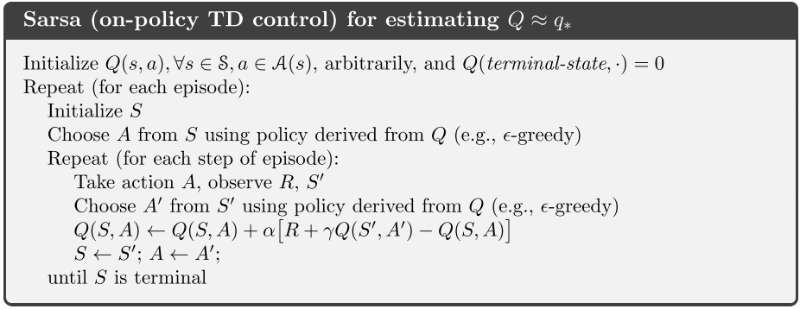
\includegraphics[width=0.7\columnwidth]{figures/sarsa-alg.jpg}
  \end{figure}

  \begin{figure}[t]
  	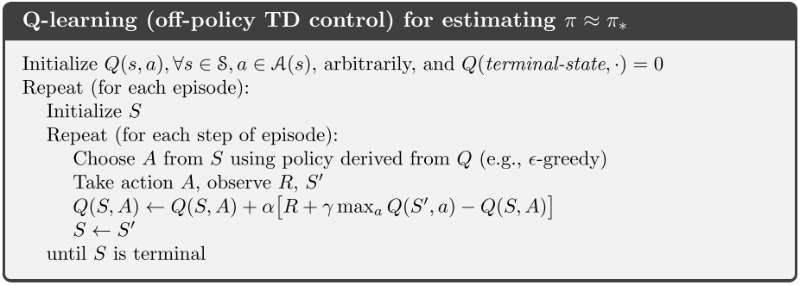
\includegraphics[width=0.7\columnwidth]{figures/q-learning-alg.jpg}
  \end{figure}
\end{frame}

\begin{frame}{Difference}
  \begin{itemize}
  	\item Exploration
  		\begin{itemize}
  			\item Sarsa: on-policy
  			\item Q-learning: off-policy
  		\end{itemize}
  	\item Update Rule
	  	\begin{itemize}
	  		\item Sarsa
	  		\begin{equation}\nonumber
	  		\begin{aligned}
	  		& Choose~ A'~ from~ S'~ using~policy~derived~from~Q~(e.g. \epsilon-greedy) \\
	  		& Q(S,A) \leftarrow Q(S,A) + \alpha[r + \gamma Q(S', A') - Q(S,A)]
	  		\end{aligned}
	  		\end{equation}
	  		\item Q-learning
	  		\begin{equation}\nonumber
	  		Q(S,A) \leftarrow Q(S,A) + \alpha[r + \gamma \max_a Q(S', a) - Q(S,A)]
	  		\end{equation}
	  	\end{itemize}
  \end{itemize}
\end{frame}




\section{Issues in Q-learning}

\subsection{Overestimation}
\begin{frame}{Overestimation}{Preliminaries}
	Recall that
	\begin{equation}
		Q(s,a) \longleftarrow r^a_s + \gamma~\red{\max}_{\ha} Q(s', \ha)
	\end{equation}
	Repeated application of this update equation eventually yields Q-values that give rise to \blue{a policy which maximizes the expected cumulative discounted reward}
	\footnote{C. J. C. H.Watkins, Learning from Delayed Rewards. PhD thesis, King’s College, Cambridge, England, 1989.} in the look-up table case.
	
	The \red{$\max$} operation may cause some problems under the approximation scenario.
\end{frame}

\begin{frame}{Overestimation}
	Assume $Q^{approx}(\cdot)$ representing implicit target values $Q^{target}$, corrupted by a noise term $Y$ such that
	\begin{equation}\nonumber
		\qa(s',\ha) = \qt(s', \ha) + Y_{s'}^{\ha}
	\end{equation}
	
	\begin{equation}
	\begin{aligned}
		Z_s &\overset{def}{=} r_s^a + \gamma~ \max_{\ha} \qa(s', \ha) - \left( r_s^a + \gamma~  \max_{\ha} \qt(s', \ha)\right) \\
		& = \gamma~ \left( \max_{\ha} \qa(s', \ha) - \max_{\ha} \qt(s', \ha)\right)
	\end{aligned}
	\end{equation}
	
	The key observation is
	\begin{equation}\nonumber
		E[Y_{s'}^{\ha}] = 0, ~ \forall \ha ~ \overset{often}{\Longrightarrow} E[Z_s] > 0 ~.
	\end{equation}
\end{frame}

\begin{frame}{Expectation of $Z$}
	\begin{Lemma}
		Let $n$ denote the number of actions applicable at state $s'$. If all $n$ actions share the same target Q-value, i.e., $\exists q: \forall \ha: q=\qt(s', \ha)$, then the average overestimation $E[Z_s]$ is $\gamma c$ with $c \overset{def}{=} \epsilon \frac{n-1}{n+1}$.
	\end{Lemma}
	\begin{Corollary}
		$0 \leq E[Z_s] \leq \gamma c$ with $c = \epsilon \frac{n-1}{n+1}$.
	\end{Corollary}
\end{frame}


\begin{frame}{Bounds for Expected Failure of Q-learning}{Simple Assumptions}
	\begin{itemize}
		\item There is a set of goal states;
		\item Positive reward $r_{goal}$ is only recieved upon entering a goal state;
		\item $r_{goal} = 1$;
		\item The state transition function is deterministic.
	\end{itemize}

	One necessary condition for the success of Q-learning is that the sequence of Q-values $Q(s_i, a_i)$ is monotonically increasing in $i$:
	\begin{equation}
		Q(s_i, a_i) \leq Q(s_{i+1}, a_{i+1}), for~all~ i \in \{0, \ldots, L-1\}
	\end{equation}
\end{frame}

\begin{frame}{Bounds for Expected Failure of Q-learning}{Simple Assumptions}
Case 1: the learner \textit{always} overestimates Q-values by $\gamma c$.
\begin{Theorem}
	If there is maximal, repeated overestimation of magnitude $\gamma c$ along an optimal path, Q-learning is expected to fail to learn an optimal policy if $\gamma > \frac{1}{1+c}$.
\end{Theorem}
\end{frame}

\begin{frame}
Case 2: Assume that Q-learning managed to learn the \textit{last} L-1 Q-values of this optimal path correctly.

\begin{itemize}
	\item Q-values are given by iteratively discounting the final reward with the \textit{distance} to the goal state, i.e., $Q(s_{L-i}, a_{L-i}) = \gamma^i$ for $i \in \{1,\ldots,L-1\}$.
	\item \textit{Correct} Q-value $Q^{correct}(s_0, a_0)$ is $\gamma^L$.
	
	\item In order to maintain monotonicity of Q, we need to make sure that
	\begin{equation}
	\gamma^{L-1} - \gamma^L \geq \gamma c ~.
	\end{equation}
\end{itemize}
\begin{theorem}
	Under the conditions above, Q-learning is expected to fail if
	\begin{equation}
		\gamma^{L-1} - \gamma^L < \gamma c ~.
	\end{equation}
\end{theorem}
\end{frame}

\begin{frame}
	\begin{theorem}
		Under the conditions above, Q-learning is expected to fail if
		\begin{equation}
			\epsilon > \frac{n+1}{n-1}\cdot \frac{(L-2)^{L-2}}{(L-1)^{L-1}} ~.
		\end{equation}
	\end{theorem}
\end{frame}

\subsection{Double Q-learning}

\begin{frame}{Double Q-learning}{Preliminaries}
	\begin{itemize}
		\item a set of random variables $X = \{X_i, \ldots, X_M\}$
			Our interest is that
			\begin{equation}\label{eq:objective}
				\max_i E[X_i] ~,
			\end{equation}
			which is in the Q-learning update rule.
		\item $S = \cup_{i=1}^M S_i$ where $S_i$ is the subset contains samples for the variable $X_i$ and each $s \in S_i$ is i.i.d.
		\item $E[X_i] = E[\mu_i] \approx \mu_i(S) \overset{def}{=}\frac{1}{|S_i|}\sum_{s\in S_i}s$ ~, where $\mu_i$ is an unbiased estimate for the value of $E[X_i]$.
		\item $f_i^{\mu}$ is PDF and $F_i^{\mu}$ is CDF of $X_i$.
	\end{itemize}
	\begin{equation}\nonumber
		\max_i E[X_i] = \max_i \int_{-\infty}^{\infty} x ~f_i^{\mu}(x)dx ~.
	\end{equation}
\end{frame}

\begin{frame}{Double Q-learning}{Single Estimator}
An obvious way to approximate the value in Eq.~(\ref{eq:objective}) is
	\begin{equation}
		\max_i E[X_i] = \max_i E[\mu_i] \approx \max_i \mu_i(S) ~.
	\end{equation}
	\begin{itemize}
		\item Assume the maximal estimator \red{$\max_i \mu_i(S)$} is distributed as PDF $f_{max}^{\mu}$.
		\item $f_{max}^{\mu} \neq f_i^{\mu}$ but $f_{max}^{\mu}$ is dependent on $f_i^{\mu}$.
		\pause
		\item CDF $F_{max}^{\mu}(x) \overset{def}{=} P(\max_i \mu_i \leq x) = \prod_{i=1}^M P(\mu_i \leq x) \overset{def}{=} \prod_{i=1}^M F_i^{\mu}(x) ~.$
	\end{itemize}
\end{frame}

\begin{frame}{Double Q-learning}{Biased Estimation of $E[X_i]$}
	\begin{itemize}
		\item The value $\max_i \mu_i(S)$ is an unbiased estimate for $E[\max_j \mu_j]$.
	\end{itemize}
	\begin{equation}
	\begin{aligned}
		E[\max_i \mu_i] &= \int_{-\infty}^{\infty} x ~f_{max}^{\mu}(x) \\
		&= \int_{-\infty}^{\infty}x\frac{d}{dx}\prod_{i=1}^M F_i^{\mu}(x)dx \\
		&= \sum_j^M \int_{-\infty}^{\infty}x ~f_j^{\mu}(s) \prod_{i\neq j}^M F_i^{\mu}(x)dx ~.
	\end{aligned}
	\end{equation}
	\begin{itemize}
		\item $\red{E}[\blue{\max}_i \mu_i]$ is not the same as $\blue{\max}_i \red{E}[X_i]$.
	\end{itemize}
\end{frame}

\begin{frame}{Double Q-learning}{Double Estimators}
	\begin{itemize}
		\item Two sets of estimators: $\mu^A={\mu_1^A,\ldots,\mu_M^A}$, $\mu^b={\mu_1^B,\ldots,\mu_M^B}$.
		\item Two subsets of samples: $S=S^A\cup S^B,~S^A \cap S^B = \emptyset$
	\end{itemize}
\end{frame}


\subsection{Averaged Q-learning}



\section{Convergence of Tabular TD}
\subsection{Sarsa}
\subsection{Q-learning}




\section{Deep Q-network}

\subsection{Nature DQN}
\subsection{Several Imrovements}


\end{document}


